\addcontentsline{toc}{section}{Introduction}
\section*{Introduction}
Ce chapitre se focalise sur l’introduction de l’entreprise d’accueil ainsi que sur la contextualisation du projet. Il débutera par une présentation de l’entreprise hôte et de ses domaines d’activité. Ensuite, nous aborderons la formulation de la problématique, les objectifs du projet, et enfin, nous discuterons de la méthodologie de gestion de projet et de sa planification.

\section{Présentation de l'organisme d'accueil}
Cette première partie présente le groupe Inetum, ses chiffres clés ainsi que sa structure organisationnelle à l'échelle internationale et nationale.

\subsection{Le Groupe Inetum}
Inetum est une ESN (Entreprise de Services du Numérique) agile, une société de
services et de solutions digitales, et un groupe international qui aide les entreprises et
les institutions à tirer le meilleur du digital flow. Aussi acteur européen de référence des
services informatiques à valeur ajoutée et des logiciels.\\
À l’international, le Groupe compte 20 filiales en France, Belgique, Luxembourg,
Suisse, Espagne, Portugal, Angleterre, Pologne, Roumanie, Singapour, Dubaï, Maroc,
Côte d’ivoire, Cameroun, Angola, Brésil, Colombie, Mexique, USA, Pérou et Panama.
Avec son profil de multi-spécialiste, Inetum met au service de ses clients une combinaison
unique de proximité, d’organisation sectorielle et de solutions de qualité industrielle. Le
groupe qui compte plus de 28.000 collaborateurs a réalisé en 2024 un chiffre d’affaires de
2,5 M€. Elle est implantée dans toute la France autour de trois grandes régions et avec
plus de 40 agences.\\
Le tableau ci-dessous regroupe les informations d'identité et les chiffres clés du groupe au niveau mondial et local :

\begin{table}[H]
    \centering
    \renewcommand{\arraystretch}{1.3}
    \begin{tabular}{|l|p{9cm}|}
        \hline
        % Ajout de \textcolor{white} ici
        \rowcolor{iNavy} \multicolumn{2}{|c|}{\textbf{\textcolor{white}{Fiche d'identité globale}}} \\ \hline
        \textbf{Date de création} & 1970 \\ \hline
        \textbf{Direction} & Vincent ROUAIX, Président-directeur Général \\ \hline
        \textbf{Siège social} & 145, Boulevard Victor Hugo, 93 400 Saint-Ouen, FRANCE \\ \hline
        \textbf{Actionnariat} & Bain Capital Private Equity (Majoritaire depuis 2022) \\ \hline
        % Ajout de \textcolor{white} ici
        \rowcolor{iNavy} \multicolumn{2}{|c|}{\textbf{\textcolor{white}{Chiffres clés 2024}}} \\ \hline
        \textbf{Chiffre d'affaires} & 2,5 Md€ (Global) / 40 M€ (Maroc) \\ \hline
        \textbf{Effectifs} & 28 000 (Monde) / +800 (Maroc) \\ \hline
        \textbf{Présence} & 19 pays, 130 bureaux \\ \hline
    \end{tabular}
    \caption{Identité et chiffres clés d'Inetum}
    \label{tab:identite_inetum}
\end{table}

\subsection{Inetum Offshore Maroc (IOM)}
Filiale à 100\% d'Inetum, Inetum Offshore Maroc est le vecteur de développement du Groupe dans les pays francophones du continent africain. Elle est le leader incontesté au Maroc en matière d’intégration et de mise en œuvre de progiciels de gestion. 

IOM met à la disposition des entreprises, ses consultants métiers et son
savoir-faire et propose à ses clients un service complet qui couvre toutes les phases du
cycle de vie des projets :
\begin{itemize}
    \setlength\itemsep{0.1em}  % Réduit l'espace entre les lignes
    \setlength\parskip{0pt}    % Supprime l'espace de paragraphe
    \setlength\parsep{0pt}     % Supprime l'espace entre les blocs
    \item[---] Conseil,
    \item[---] Conception,
    \item[---] Intégration,
    \item[---] Formation,
    \item[---] Déploiement et Maintenance.
\end{itemize}

Le tableau suivant représente la fiche technique d’Inetum Offshore Maroc, qui résume toutes ses informations :
\begin{table}[H]
    \centering
    \renewcommand{\arraystretch}{1.3}
    \begin{tabular}{|l|p{9cm}|}
        \hline
        \textbf{Date de création} & 2011 \\ \hline
        \textbf{Direction} & OUALI Fouzia \\ \hline
        \textbf{Taille de l’entreprise} & ~1000 collaborateurs \\ \hline
        \textbf{Siège social} & Casa Nearshore Parc, Shore 28. 100, Bd. Al Qods, Sidi Maârouf, Casablanca \\ \hline
        \textbf{Forme juridique} & Société Anonyme (SA) \\ \hline
        \textbf{Capitale} & 400 000 DHS \\ \hline
    \end{tabular}
    \caption{Fiche technique d’Inetum Offshore Maroc}
    \label{tab:fiche_iom}
\end{table}

\subsection{Organisation et pôles d'expertise}
Inetum structure son expertise autour de quatre "Global Business Lines" (GBL) majeures :

\begin{itemize}
    \setlength\itemsep{0.1em}  % Réduit l'espace entre les lignes
    \setlength\parskip{0pt}    % Supprime l'espace de paragraphe
    \setlength\parsep{0pt}
    \item \textbf{Inetum Consulting (2\% du CA) :} Conseil en stratégie digitale et IA.
    \item \textbf{Inetum Technologies (64\% du CA) :} Gestion des infrastructures, Cloud et Cybersécurité.
    \item \textbf{Inetum Solutions (26\% du CA) :} Intégration d'ERP (SAP, Microsoft, Sage).
    \item \textbf{Inetum Software (8\% du CA) :} Édition de logiciels verticaux.
\end{itemize}

\subsection{Secteurs d’activité}
Inetum est l’un des leaders mondiaux dans le domaine du conseil, des services infor
matiques et de l’infogérance. Les métiers du groupe s’organisent en 6 grandes disciplines 

\begin{itemize}
    \setlength\itemsep{0.1em}  % Réduit l'espace entre les lignes
    \setlength\parskip{0pt}    % Supprime l'espace de paragraphe
    \setlength\parsep{0pt}
    \item \textbf{Conseil :} Accompagnement stratégique.
    \item \textbf{Services applicatifs et d’infrastructures :} Support et développement.
    \item \textbf{Intégration systèmes :} Business Solutions, ERP, CRM.
    \item \textbf{Outsourcing :} Infogérance et gestion externe.
    \item \textbf{Value Added Reselling :} Revente de solutions à valeur ajoutée.
    \item \textbf{Software :} Solutions verticales (Assurances, Santé) et transverses (Chronotime).
\end{itemize}

Le groupe intervient dans l’ensemble des secteurs, pour répondre aux besoins de ses
clients et leur proposer les solutions les mieux adaptées à leurs métiers spécifiques. Le
groupe dispose d’une stratégie pertinente et d’un savoir-faire très solide pour développer
ses relations clients dans plusieurs secteurs.

\begin{figure}[H]
    \centering
    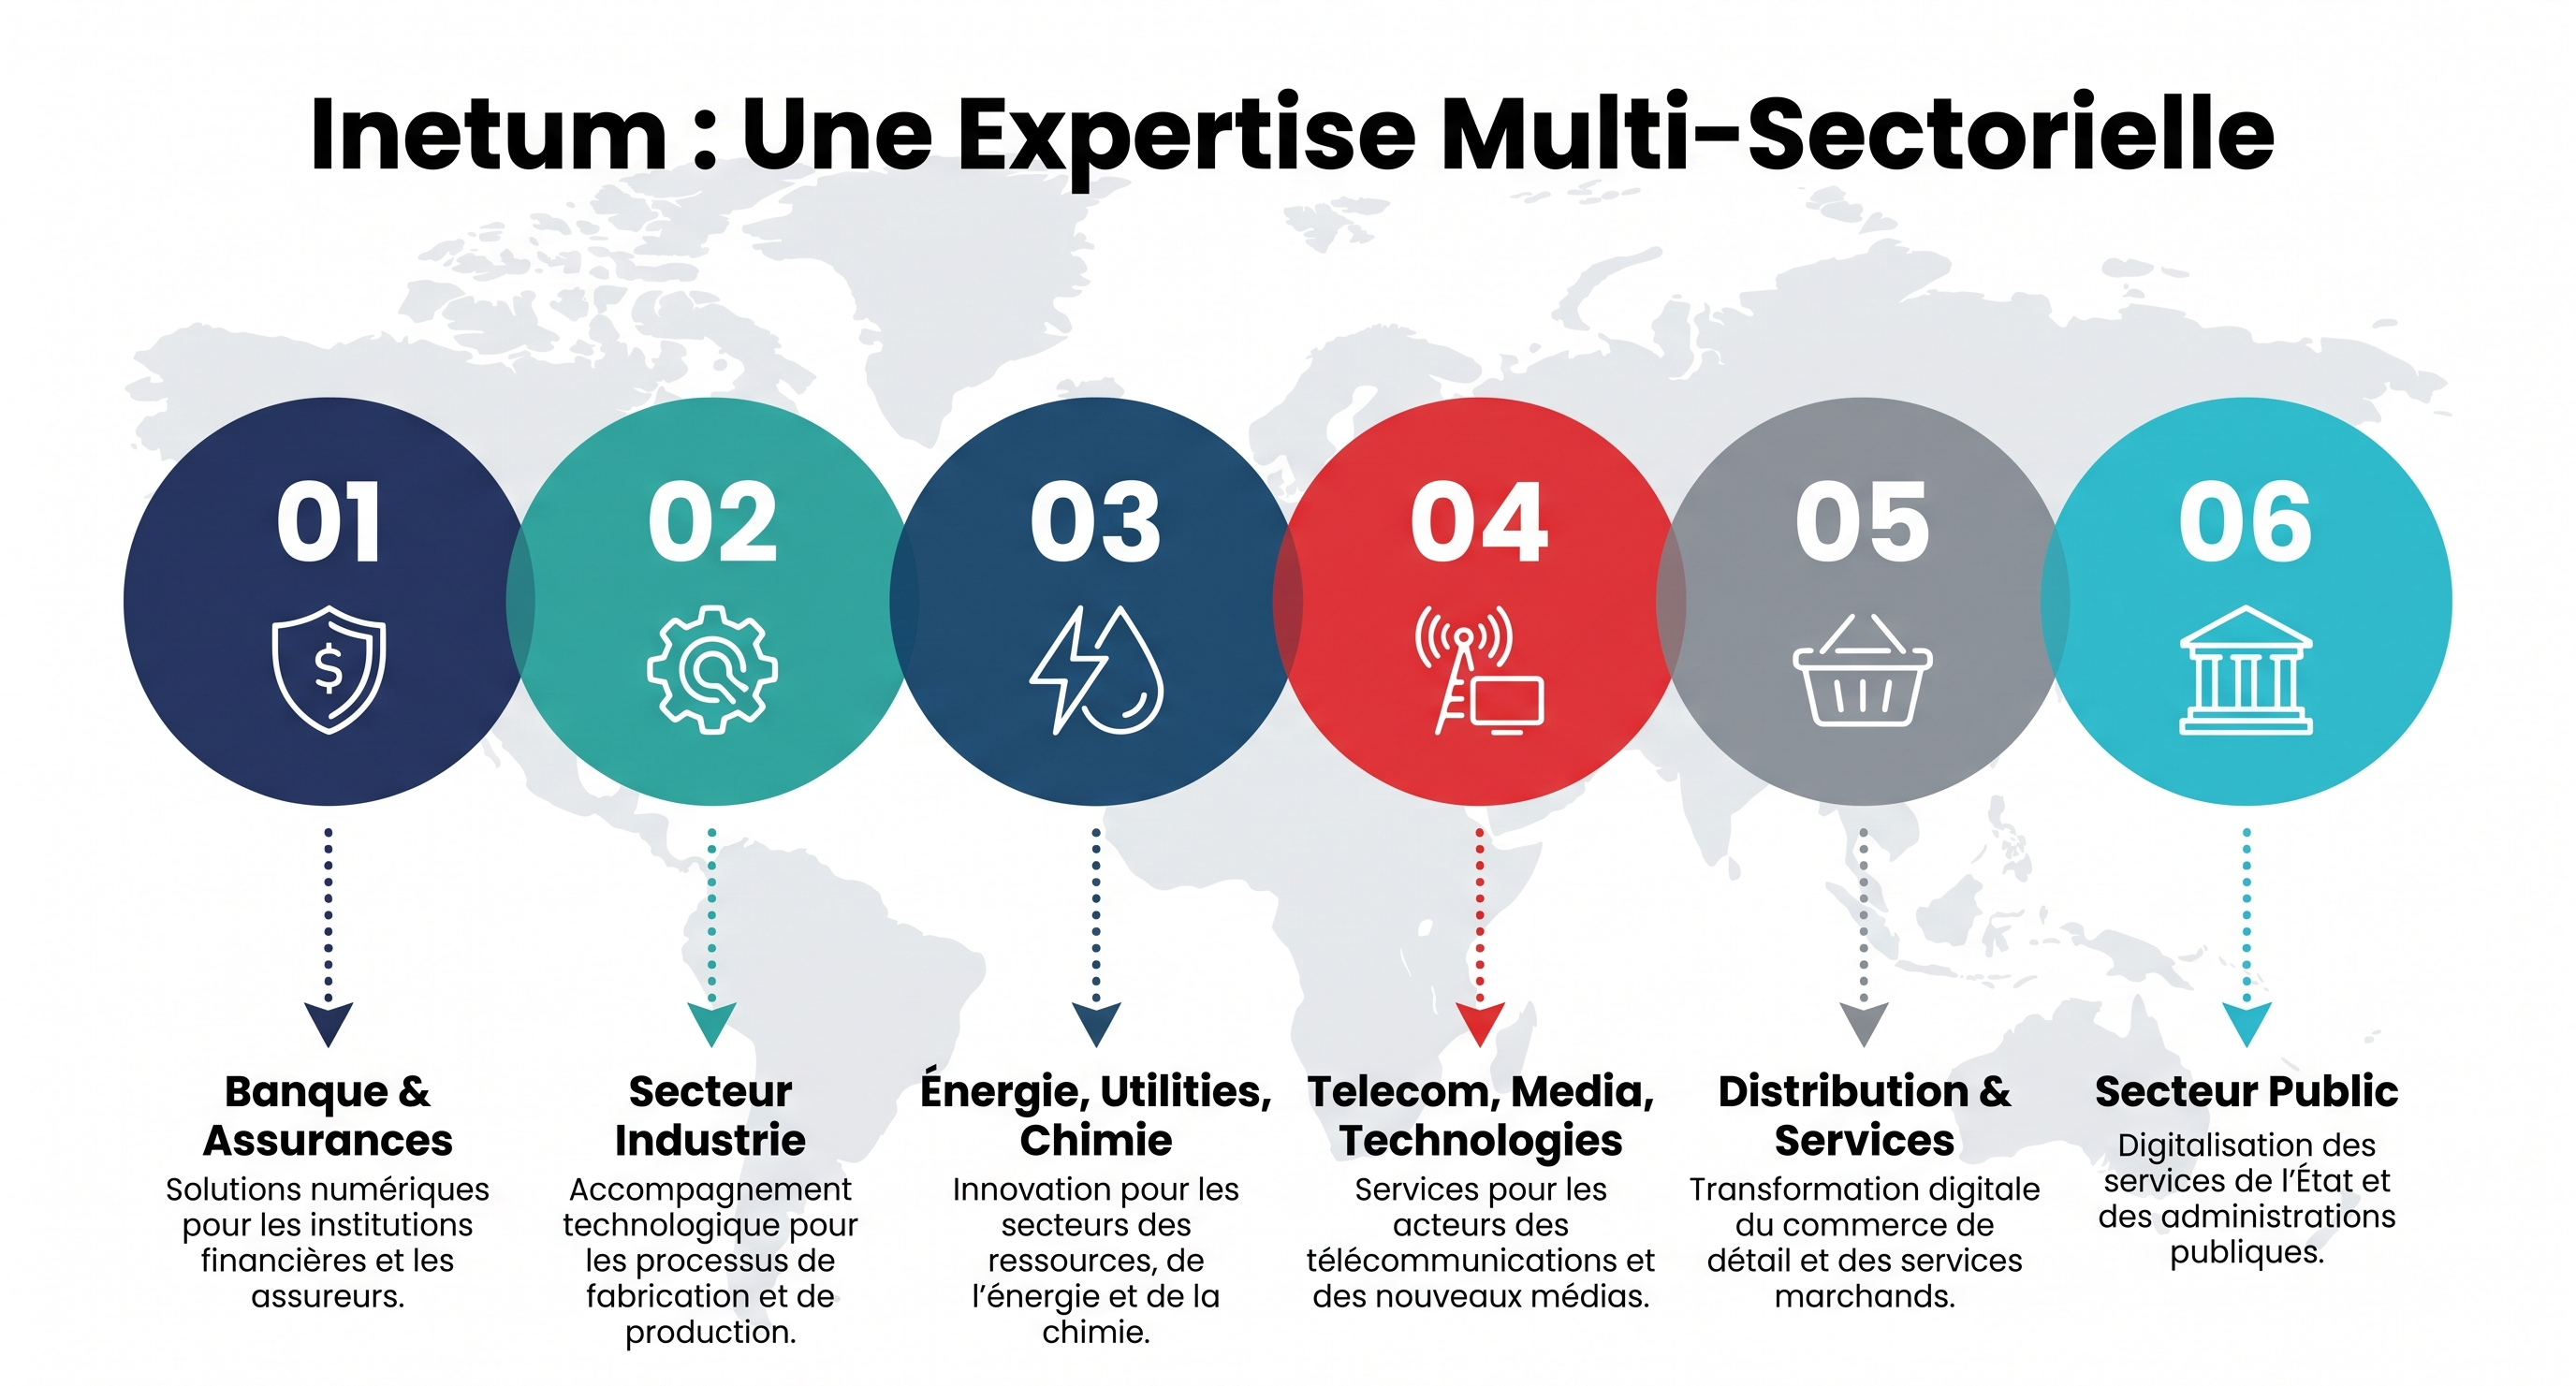
\includegraphics[width=0.9\textwidth]{images/secteur d'activite.png}
    \caption{Secteurs d'activité}
    \label{fig:secteurs}
\end{figure}



\subsection{Organigramme d'Inetum Offshore Maroc}
Dans le cadre de notre projet, il est essentiel de bien comprendre la structure organisationnelle de l’équipe projet. L’organigramme joue un rôle crucial en définissant les rôles et responsabilités de chaque membre, en facilitant la communication et en assurant une coordination efficace des tâches. Cet organigramme permet également de clarifier les relations hiérarchiques et fonctionnelles au sein de l’équipe. 

L’organigramme détaillé du projet est présenté dans la figure~\ref{fig:org_projet} :

\begin{figure}[H]
    \centering
    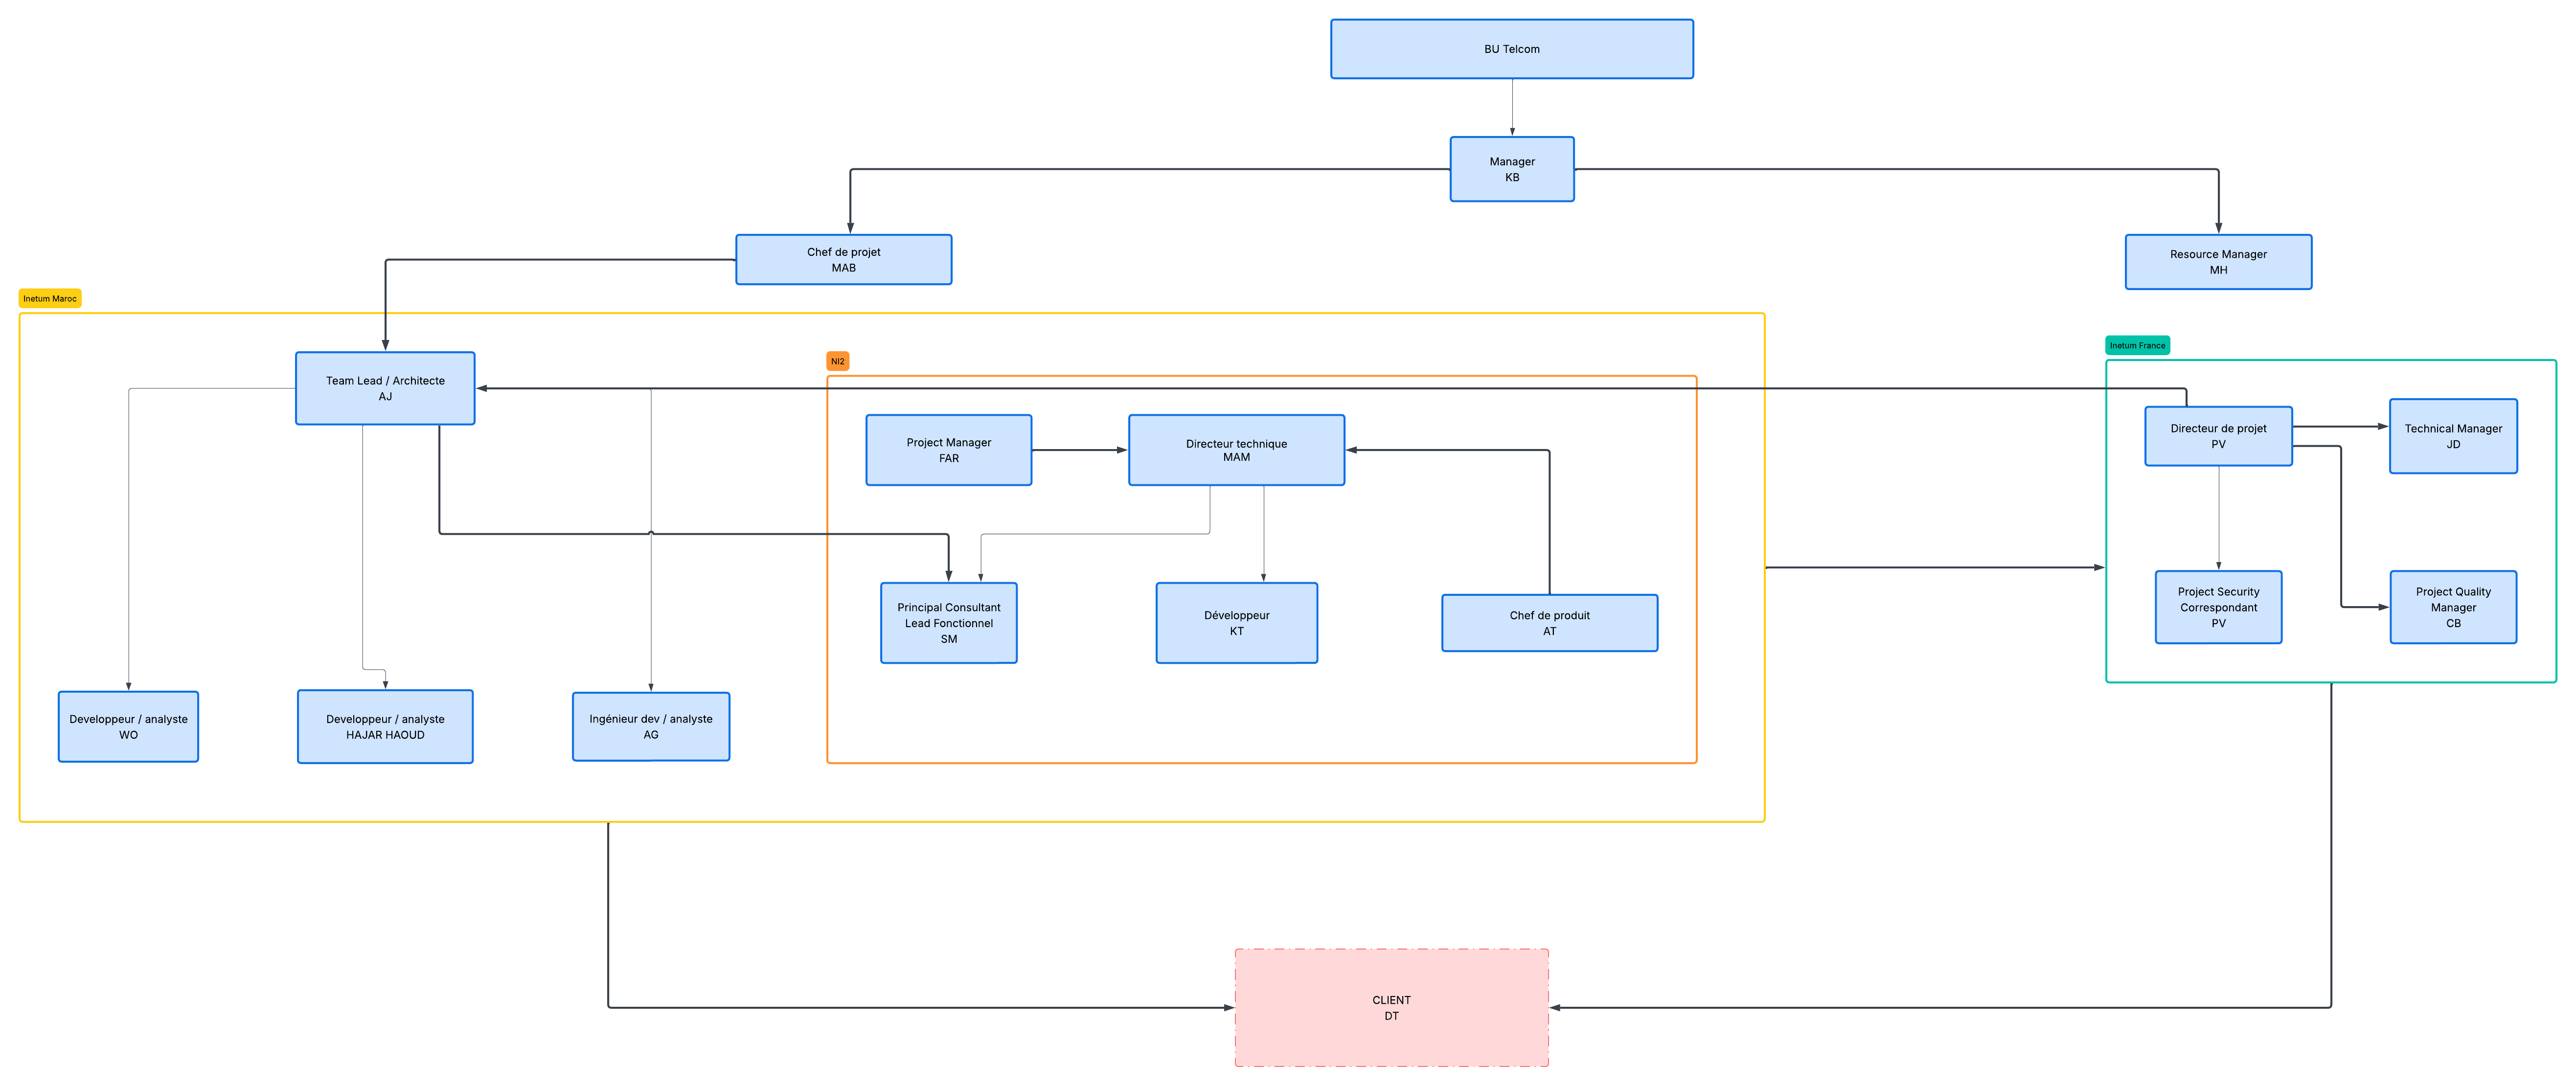
\includegraphics[width=0.9\textwidth]{images/organigramme3.png}
    \caption{Organigramme d'Inetum Offshore Maroc} 
    \label{fig:org_projet} 
\end{figure}


\subsection{Partenaires et Clients}

Inetum collabore avec des partenaires technologiques de premier plan afin d’enrichir son offre de services et de répondre efficacement aux besoins de ses clients. Grâce à cette stratégie et à son expertise locale, plus de 500 entreprises marocaines lui font confiance pour les accompagner dans leur transformation digitale.

\paragraph{Partenaires stratégiques :}
\begin{itemize}
    \setlength\itemsep{0.1em}  % Réduit l'espace entre les lignes
    \setlength\parskip{0pt}    % Supprime l'espace de paragraphe
    \setlength\parsep{0pt}
    \item \textbf{SAP :} Solutions ERP pour la gestion d’entreprise.
    \item \textbf{Microsoft :} Technologies cloud et bureautique.
    \item \textbf{Oracle :} Bases de données et logiciels métiers.
    \item \textbf{IBM :} Services IT, IA et infrastructure.
\end{itemize}

\paragraph{Principaux clients au Maroc :}
\begin{itemize}
    \setlength\itemsep{0.1em}  % Réduit l'espace entre les lignes
    \setlength\parskip{0pt}    % Supprime l'espace de paragraphe
    \setlength\parsep{0pt}
    \item \textbf{OCP :} Leader mondial dans le secteur des phosphates.
    \item \textbf{ONCF :} Opérateur national du transport ferroviaire.
    \item \textbf{Allianz :} Compagnie d’assurance internationale.
    \item \textbf{Royal Air Maroc :} Compagnie aérienne nationale.
\end{itemize}


\medskip
\vspace{15cm}

\section{Contexte du projet}

\subsection{Cadre général du projet}
Dans un secteur des télécommunications en constante mutation, les opérateurs doivent moderniser leur Système d'Information (SI) Commercial pour répondre aux attentes des clients et soutenir le déploiement de nouvelles technologies (FTTH, 4G/5G). Le programme de refonte porte sur le système \textbf{CCU} (Commande et Catalogue Unifiés), qui centralise le catalogue de produits et la gestion des commandes clients.

\medskip

Le projet objet de ce mémoire ne porte pas sur la migration de données, mais sur la conception d'un \textbf{agent IA de diagnostic technique} capable d'assister les équipes de support dans la résolution des incidents affectant le SI CCU. L'agent exploite les APIs \textbf{TMF620} (Product Catalog) et \textbf{TMF622} (Product Ordering) du TM Forum pour s'aligner sur les standards de l'industrie télécom.

\subsection{Problématique et enjeux}
Les équipes de support technique font face à des incidents dont l'investigation requiert de consulter plusieurs sources disjointes :

\begin{itemize}
    \setlength\itemsep{0.1em}
    \setlength\parskip{0pt}
    \setlength\parsep{0pt}
    \item Les \textbf{logs réseau} et applicatifs, souvent volumineux et difficiles à interpréter rapidement.
    \item Le \textbf{contexte client} stocké dans le CRM (statut du contrat, services actifs, historique).
    \item Les \textbf{tickets historiques} résolus, qui contiennent une expertise précieuse mais sont difficiles à exploiter manuellement.
\end{itemize}

Cette dispersion des données engendre des temps de diagnostic longs, une dépendance forte à l'expertise humaine et un risque d'erreur. La problématique centrale est donc la suivante : \textbf{comment concevoir un système intelligent capable de corréler automatiquement ces sources pour produire un diagnostic fiable, explicable et actionnable, sans jamais exécuter d'action corrective automatique sur le SI réel ?}

\subsection{Périmètre fonctionnel}
Le périmètre du projet couvre les fonctionnalités suivantes :

\begin{enumerate}
    \item \textbf{Intake intelligent} : normalisation d'un incident exprimé en langage naturel ou structuré.
    \item \textbf{Collecte multi-source} : récupération parallèle des logs, du contexte client et des tickets similaires.
    \item \textbf{Raisonnement sur la cause racine} : corrélation des sources avec attribution d'un niveau de confiance.
    \item \textbf{Gestion des tickets} : mapping ou création d'un ticket dans l'outil de ticketing (Zammad).
    \item \textbf{Remédiation explicative} : proposition d'actions informatives (non exécutables automatiquement).
    \item \textbf{Guardrail de contenu} : vérification PII avant envoi externe.
    \item \textbf{Génération de rapport} : production d'un rapport PDF/HTML.
    \item \textbf{Notification} : envoi d'email et ajout d'une note dans le ticket.
\end{enumerate}

\subsection{Objectifs du projet}
Les objectifs du projet se déclinent en quatre axes :

\begin{itemize}
    \setlength\itemsep{0.1em}
    \setlength\parskip{0pt}
    \setlength\parsep{0pt}
    \item \textbf{Centraliser l'investigation} : offrir un point d'entrée unique qui agrège les sources pertinentes à un incident.
    \item \textbf{Fiabiliser le diagnostic} : réduire les erreurs humaines grâce à une corrélation structurée et à un raisonnement guidé par les données.
    \item \textbf{Capitaliser l'expertise} : exploiter les tickets historiques via un graphe de connaissances et une recherche sémantique.
    \item \textbf{Garantir la sécurité} : s'assurer qu'aucune action technique n'est exécutée automatiquement et que les données sensibles sont filtrées.
\end{itemize}

\section{Méthodologie et planification}

\subsection{Choix méthodologique}
La conduite du projet s'appuie sur une approche hybride combinant le cycle en V pour la gouvernance globale et la méthode Agile/Scrum pour l'itération technique. Cette approche permet de concilier rigueur de spécification et capacité d'adaptation face à la complexité des systèmes legacy et des modèles d'IA.

Le développement a été découpé en sprints de deux à quatre semaines, avec les rituels suivants :

\begin{itemize}
    \setlength\itemsep{0.1em}
    \setlength\parskip{0pt}
    \setlength\parsep{0pt}
    \item \textbf{Backlog produit} : centralisation des fonctionnalités (agents, API, ingestion, tests).
    \item \textbf{Sprints thématiques} : intake, collecteurs, raisonnement, guardrail, reporting, notification.
    \item \textbf{Daily stand-ups} : synchronisation rapide avec les encadrants et l'équipe technique.
    \item \textbf{Démos et rétrospectives} : validation des livrables et amélioration continue.
\end{itemize}

\subsection{Planification}
Le tableau \ref{tab:planning} résume les grandes phases du projet.

\begin{table}[H]
    \centering
    \renewcommand{\arraystretch}{1.3}
    \begin{tabular}{|l|p{8cm}|l|}
        \hline
        \rowcolor{iNavy} \textbf{\color{white}Phase} & \textbf{\color{white}Description} & \textbf{\color{white}Durée} \\ \hline
        Analyse & Étude du SI CCU, APIs TMF et sources de données & 2 semaines \\ \hline
        Conception & Architecture agentique, modèle de données Neo4j, flux & 3 semaines \\ \hline
        Réalisation & Implémentation des agents, API, ingestion & 5 semaines \\ \hline
        Validation & Tests pytest, golden incidents, recette & 2 semaines \\ \hline
        Documentation & Rédaction du rapport et démonstration & 2 semaines \\ \hline
    \end{tabular}
    \caption{Planification macro du projet}
    \label{tab:planning}
\end{table}

\section*{Conclusion}
Ce premier chapitre a présenté le contexte général du projet, l'organisme d'accueil, la problématique du diagnostic technique CCU, les objectifs et la méthodologie adoptée. Le chapitre suivant détaille la conception de l'architecture agentique et du graphe de connaissances.
